\documentclass[10pt,twocolumn]{article}
\usepackage[margin=0.9in]{geometry}
\usepackage{graphicx}
\usepackage{booktabs}
\usepackage{amsmath}
\usepackage{url}
\usepackage[hidelinks]{hyperref}
\usepackage{xspace}

\newcommand{\trainable}{\textsc{Trainable}\xspace}
\newcommand{\practical}{\textsc{Practical}\xspace}
\newcommand{\loadable}{\textsc{Loadable}\xspace}
\newcommand{\efficient}{\textsc{Efficient}\xspace}

\title{How Far Can 16\,GB Go? Characterizing Memory-Efficient LLM Fine-Tuning\\ on Consumer Apple Silicon}
\author{Anonymous}
\date{September 2026}

\begin{document}
\maketitle

\begin{abstract}
% Filled after formal data is generated; every number traced to results/raw/.
PLACEHOLDER-ABSTRACT
\end{abstract}

\section{Introduction}
PLACEHOLDER-INTRO

\section{Background and Related Work}
\label{sec:related}
\subsection{Apple Silicon and Unified Memory}
Apple Silicon SoCs present a single physical memory pool shared by CPU and GPU.
\texttt{mlx}~\cite{mlx2023} is an array framework that targets this architecture
directly; \texttt{mlx-lm}~\cite{mlxlm} provides LLM fine-tuning on top of it.
Prior profiling of Apple Silicon training reports substantial gaps to NVIDIA
GPUs and identifies page faults and kernel-launch overhead as system-level
contributors~\cite{feng2025profiling}. Benchmarking of MLX itself has so far
focused on inference latency for encoder models~\cite{ajayi2025benchmarking};
consumer-device LLM stacks beyond MLX include llama.cpp~\cite{llamacpp}.

\subsection{MLX}
The MLX framework exposes Metal-backed computation with lazy evaluation and a
composable optimizer API~\cite{mlx2023}. Our measurement validation
(Sec.~\ref{sec:measurements}) quantifies why explicit synchronization is
required for per-step timing under lazy execution.

\subsection{LoRA and QLoRA}
LoRA~\cite{hu2022lora} parameterizes weight updates with low-rank adapters;
QLoRA~\cite{dettmers2023qlora} backpropagates through 4-bit quantized frozen
weights, following the broader line of LLM quantization
work~\cite{dettmers2022llmint8}. Both reduce the memory footprint relative to
full fine-tuning~\cite{houlsby2019parameter,chen2016training}, and
GaLore~\cite{zhao2024galore} targets the same budget from the optimizer-state
side. These methods are largely evaluated on data-center GPUs; how they behave
inside a 16\,GB unified-memory budget is the subject of this paper.

\subsection{Resource-Constrained LLM Fine-Tuning}
Prior systems work has profiled Apple Silicon for ML training
end-to-end~\cite{feng2025profiling} and benchmarked MLX inference for encoder
models~\cite{ajayi2025benchmarking}, but the fine-tuning feasibility boundary
on a fixed consumer unified-memory budget --- which model scales, precisions,
and context lengths admit \emph{completed} training steps, and at what cost ---
has not, to our knowledge, been mapped by a preregistered benchmark. Closest
in spirit, memory-efficiency methods such as GaLore~\cite{zhao2024galore} and
QLoRA~\cite{dettmers2023qlora} report feasibility on GPU hardware where
CPU/GPU memory are separate; unified memory changes the failure mode (page
thrumbling rather than allocator exceptions), which motivates our measurement
design.

\section{Methodology}
\label{sec:method}
\subsection{Research Questions}
We study:
\begin{itemize}
  \item \textbf{RQ1} How do memory, step time, and throughput of BF16 LoRA and
        4-bit QLoRA scale with model size?
  \item \textbf{RQ2} How far does 4-bit quantization extend the
        \trainable boundary?
  \item \textbf{RQ3} Where is the context-length boundary?
  \item \textbf{RQ4} Does the memory saving of quantization come with a
        measurable training-time penalty?
  \item \textbf{RQ5} How large is the gap between ``training can start'' and
        \practical fine-tuning?
\end{itemize}

\subsection{Hardware and Software}
All experiments run on a single Apple Mac mini with an Apple M4 SoC, 16\,GiB
unified memory, and macOS~26.5; the exact preflight-recorded environment is in
Table~\ref{tab:setup}. Software was locked with uv: Python~3.13.11,
\texttt{mlx}~0.32.2, \texttt{mlx-lm}~0.31.3. The M4 generation context is from
Apple's release material~\cite{applem4}.

\subsection{Models}
We use the Qwen3 family~\cite{yang2025qwen3}: instruction-tuned chat models
(not base models) at 0.6B/1.7B/4B in BF16 and 0.6B--14B as pre-quantized 4-bit
mlx-community conversions; every repository is pinned to a Hub revision and
byte-verified (Table~\ref{tab:setup}).

\subsection{Dataset}
The formal benchmark uses a frozen subset of
ultrachat\_200k~\cite{ding2023ultrachat} (revision \texttt{8049631c}): 2{,}048
training and 32 validation conversations sampled with seed 42 and formatted
with the Qwen3 chat template; loss is a standard LM loss over all tokens.
The manifest and SHA-256 sums ship with the repository. Synthetic long-context
workloads are used only for context-scaling systems analysis, never for
quality claims.

\subsection{Fine-Tuning Methods}
BF16 LoRA (rank 8, $\alpha$=16, dropout 0, targets q/k/v/o\_proj), 4-bit QLoRA
(same adapters, group size 64), and, for the smallest model only, full
fine-tuning. Optimizer AdamW, lr $10^{-4}$, constant schedule, micro-batch 1.

\subsection{Measurement Methodology}
\label{sec:measurements}
Every run is launched by an Experiment Supervisor that records git provenance,
hardware, memory/swap state (before, after, and 1\,Hz sampling), full
stdout/stderr, per-step timings, and an atomic SHA-256 manifest; failures are
first-class results. Step timing includes forward, backward, optimizer update,
and an explicit \texttt{mx.eval} synchronization; we measured that omitting
this synchronization under-reports step time by three orders of magnitude
under MLX's lazy execution. Peak memory is the MLX allocator's Metal-buffer
high-water mark (\texttt{get\_peak\_memory}); it is not process RSS, and on
unified memory it may exceed physical RAM, at which point macOS paging carries
the excess. Full validation evidence is in the repository
(\texttt{docs/measurement\_validation.md}).

\subsection{Operational Definitions}
\label{sec:definitions}
\loadable: the training process loads the model weights.
\trainable: the run completes every requested optimizer step with
\texttt{terminal\_state=success} and no kill signal.
\practical: \trainable and (P1) sampled peak system swap does not exceed the
pre-run level by more than 4\,GiB, and (P2) median step time $\le$10\,s.
\efficient: \practical with throughput $\ge$100 loss-bearing tokens/s.
All thresholds were frozen before any formal run
(research/preregistration.md); we report sensitivity to $\pm 2\times$
threshold changes. SIGKILL terminations are never reclassified as OOM without
direct kernel evidence.

\subsection{Reproducibility}
Formal configurations, the dataset freeze, the analysis pipeline, and this
paper's tables and figures are generated from raw results by committed scripts;
no number is hand-typed. Appendix~\ref{app:repro} lists reproduction commands.

\section{Results}
\subsection{Model-Scale Feasibility}
PLACEHOLDER-SCALE-FEASIBILITY
\begin{table*}[t]\centering
\caption{Formal benchmark at ctx=512, b1-ga1, rank 8, lr 1e-4, 100 steps, preregistered seeds \{42,123,2026\} (mean$\pm$SD over completed seeds; memory is MLX allocator peak; $\pm$0.00 marks bit-identical allocator peaks across seeds; D1/D8 cells are regime-dependent boundary observations discussed in the text; 95\% $t$-CIs in Table~\ref{tab:ci}).}
\label{tab:matrix}
\footnotesize\setlength{\tabcolsep}{4pt}
\begin{tabular}{llrrrrr}
\toprule
Model & Method & Seeds & Peak mem (GiB) & Median step (s) & Tok/s & Val loss\\
\midrule
Qwen3-0.6b (0.6B) & Full FT & 3/3 & 5.77$\pm$0.00 GiB & 1.081$\pm$0.003 & 428.6$\pm$49.9 & 4.441$\pm$0.147\\
Qwen3-0.6b (0.6B) & BF16 LoRA & 3/3 & 2.92$\pm$0.00 GiB & 0.619$\pm$0.009 & 809.9$\pm$9.2 & 1.813$\pm$0.002\\
Qwen3-1.7b (1.7B) & BF16 LoRA & 3/3 & 5.55$\pm$0.00 GiB & 1.396$\pm$0.005 & 366.2$\pm$2.5 & 1.549$\pm$0.001\\
Qwen3-4b (4.0B) & BF16 LoRA & 1/3 (D1) & 11.54 GiB & 3.028 & 168.1 & 1.431\\
Qwen3-0.6b (0.6B) & 4bit QLoRA & 3/3 & 2.13$\pm$0.00 GiB & 0.697$\pm$0.003 & 721.4$\pm$4.0 & 1.926$\pm$0.001\\
Qwen3-1.7b (1.7B) & 4bit QLoRA & 3/3 & 3.30$\pm$0.00 GiB & 1.697$\pm$0.006 & 300.9$\pm$1.1 & 1.634$\pm$0.011\\
Qwen3-4b (4.0B) & 4bit QLoRA & 3/3 & 6.19$\pm$0.00 GiB & 3.665$\pm$0.007 & 137.2$\pm$1.1 & 1.472$\pm$0.001\\
Qwen3-8b (8.2B) & 4bit QLoRA & 3/3 & 9.19$\pm$0.00 GiB & 10.039$\pm$0.006 & 42.9$\pm$1.1 & 1.377$\pm$0.007\\
Qwen3-14b & 4bit QLoRA & 0/3 (D8) & -- & -- & -- & --\\
\bottomrule
\end{tabular}
\end{table*}


\subsection{Memory Scaling}
PLACEHOLDER-MEMORY-SCALING

\begin{figure}[t]
  \centering
  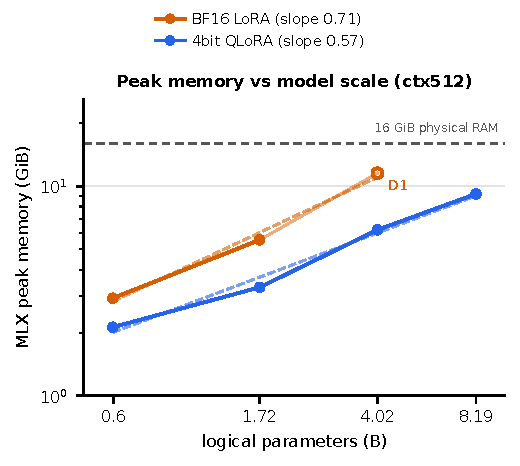
\includegraphics[width=\columnwidth]{../results/figures/fig3_memory_scaling.pdf}
  \caption{Peak memory vs.\ model scale at ctx=512 (mean$\pm$SD of three
  seeds). Fits are log-log least squares over the plotted points.}
  \label{fig:memscale}
\end{figure}

\subsection{Training-Time Scaling}
PLACEHOLDER-TIME-SCALING

\subsection{Quantization Trade-offs}
PLACEHOLDER-QUANT-TRADEOFFS
\begin{table}[t]\centering
\caption{Paired quantization effects (same model/seed; ratios = 4bit/BF16). Timing equivalence margin $\pm$25\% frozen before benchmark.}
\label{tab:paired}
\small
\begin{tabular}{lrrr}
\toprule
Model & Mem ratio & Step-time ratio & Tok/s ratio\\
\midrule
Qwen3-0.6b & 0.73 & 1.13 & 0.89\\
Qwen3-1.7b & 0.59 & 1.22 & 0.82\\
Qwen3-4b & 0.54 & 1.21 & 0.81\\
\bottomrule
\end{tabular}
\end{table}


\subsection{Context-Length Boundary}
PLACEHOLDER-CONTEXT-BOUNDARY

\begin{figure}[t]
  \centering
  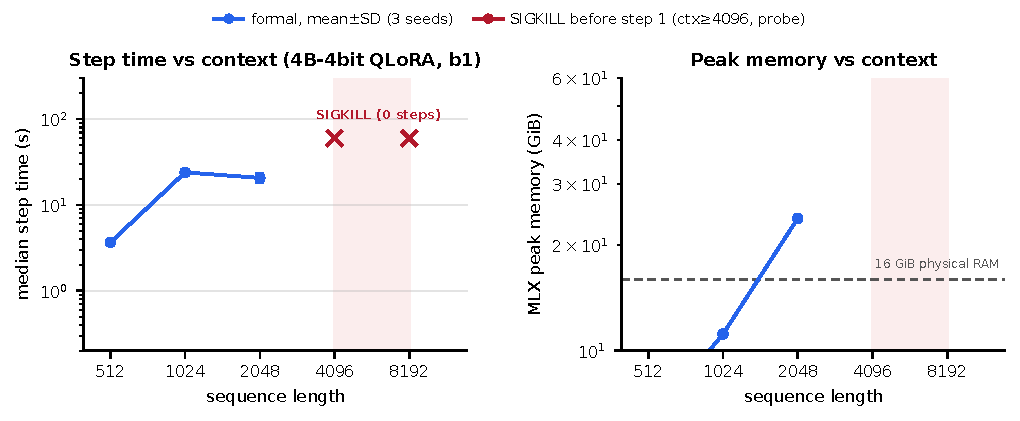
\includegraphics[width=\columnwidth]{../results/figures/fig5_context_scaling.pdf}
  \caption{Context scaling for 4B 4-bit QLoRA: step time (left) and peak
  memory (right). Crosses mark SIGKILL probe failures; shaded region marks the
  failure interval.}
  \label{fig:ctx}
\end{figure}

\subsection{Training Effectiveness}
PLACEHOLDER-EFFECTIVENESS

\section{Failure Analysis}
PLACEHOLDER-FAILURE-ANALYSIS
\begin{table*}[t]\centering
\caption{Failure taxonomy over all 27 failed runs (terminal states preserved verbatim; categories are evidence-based labels, never reclassifications).}
\label{tab:failures}
\footnotesize\setlength{\tabcolsep}{4pt}
\begin{tabular}{p{3.0cm}rp{3.4cm}p{7.0cm}}
\toprule
Category & Runs & Configurations & Evidence\\
\midrule
External SIGKILL (memory pressure) & 6 & qwen3-4b-4bit (b8$\times$3, ctx2048, ctx4096 [probe], ctx8192 [probe]) & exit 137 / SIGKILL, steps not recorded; kernel JetsamEvent confirms one b8 kill (App.~\ref{app:jetsam}); rest SIGKILL-consistent only, not reclassified as OOM; terminal state: runtime\_error (SIGKILL)\\
Supervisor timeout & 4 & qwen3-14b-4bit; qwen3-4b (BF16); qwen3-8b (BF16) [probe]; qwen3-8b-4bit & killed at the configured supervisor limit 2400--7200\,s under multi-GiB swap residency; terminal state: timeout (SIGKILL)\\
Operator interrupt & 5 & qwen3-0.6b (BF16); qwen3-4b (BF16)$\times$2; qwen3-4b-4bit$\times$2 & operator halt after 15--1627\,s; retained as system-state evidence (D1/D7); terminal state: user\_interrupted\\
Trainer implementation bug (D5) & 9 & qwen3-4b-4bit (b2$\times$3, b4$\times$3, b8$\times$3) & python traceback in variable-length validation batching (micro-batch $\ge$2); rerun on the fixed trainer; terminal state: runtime\_error\\
Pre-formal pipeline debug & 2 & qwen3-0.6b (BF16)$\times$2 & python traceback before the formal matrix was frozen; terminal state: runtime\_error\\
Unresolved failure & 1 & qwen3-14b-4bit & no specific pattern in exit evidence; 14B attempt attributed to operator KeyboardInterrupt per D8; terminal state: unknown\_failure\\
\bottomrule
\end{tabular}
\end{table*}


\section{Discussion}
\subsection{What Does 16 GB Actually Enable?}
PLACEHOLDER-DISCUSSION-ENABLE

\subsection{Loadable vs Trainable vs Practical}
PLACEHOLDER-DISCUSSION-LAYERS

\subsection{Implications for Consumer LLM Research}
PLACEHOLDER-DISCUSSION-IMPLICATIONS

\subsection{Limitations}
PLACEHOLDER-LIMITATIONS-DETAIL

\subsection{Ethics and Licensing}
The benchmark targets publicly released model weights (Apache~2.0 for Qwen3)
and a publicly released dataset (ultrachat\_200k, research-permitted license);
no synthetic workload contributes to quality claims. All measurements were
performed on the authors' own hardware.

\section{Conclusion}
PLACEHOLDER-CONCLUSION

\bibliographystyle{plain}
\bibliography{references}

\appendix
\section{Reproducibility Instructions}
\label{app:repro}
The repository ships the complete chain:
\begin{enumerate}
  \item \texttt{uv sync} recreates the locked Python environment.
  \item \texttt{uv run python scripts/run\_experiment.py --config <yaml> --}
        launches any experiment under the supervisor; formal configurations
        are \texttt{configs/experiments/formal/}.
  \item \texttt{data/formal\_sft\_v1/} contains the frozen dataset with
        \texttt{MANIFEST.json} and \texttt{SHA256SUMS}.
  \item \texttt{uv run python scripts/run\_analysis.py} regenerates every
        processed table, figure, and summary from \texttt{results/raw/}.
  \item Every raw result directory contains its exact command, effective
        configuration, environment snapshot, logs, and a SHA-256 manifest.
\end{enumerate}
PLACEHOLDER-APPENDIX-CONFIGS

\section{Measurement Validation}
\label{app:measurements}
Summary of \texttt{docs/measurement\_validation.md}: (A) step timing requires
the explicit \texttt{mx.eval} synchronization present in the trainer;
asynchronous dispatch under-reports step time by $\sim$4{,}500$\times$ on a
reference workload. (B) \texttt{get\_peak\_memory} counts MLX allocator
buffers in bytes; a 1\,GiB allocation increases both active and peak memory by
exactly 1\,GiB after reset. (C) All raw results are arithmetically consistent
with their per-step timing artifacts under their declared interval
definitions. (D) The 1\,Hz swap sampler consumes 1.47\% of one CPU core at
5$\times$ the formal cadence.

\end{document}
